% Companion note for the GFOL (grid-following VSC) injector model in RAMSES.
% Based on the model notes by T. Van Cutsem (July 2026) and the CODEGEN
% description file inj_GFOL.txt in the RAMSES repository.
% Compile with:  pdflatex inj_gfol.tex  (twice)
\documentclass[11pt,a4paper]{article}
\usepackage[margin=25mm]{geometry}
\usepackage{amsmath,bm}
\usepackage{graphicx}
\usepackage[T1]{fontenc}
\renewcommand{\familydefault}{\sfdefault}
\setlength{\parindent}{0pt}
\setlength{\parskip}{2ex}
\pagestyle{empty}

\begin{document}

\begin{center}
{\large\bf GFOL: Grid-following VSC modelling in RAMSES}\\[1ex]
{\small based on the model by T.\ Van Cutsem (July 2026)}
\end{center}

{\bf Overview.} An MMC-type converter connected to the grid through its
transformer (resistance $R$, inductance $L$, ideal ratio $r$; no LC filter).
The DC side is not modelled; the focus is on the AC grid dynamics. The model
is rather detailed (measurement low-pass filters, PLL with blocking
hysteresis, outer power loops, inner current control loops, dynamic voltage
support). Per-unit values refer to the nominal apparent power $S_{nom}$ of
the converter; the conversion factor of currents is $k = r\,S_{base}/S_{nom}$.

{\bf Reference frame.} The VSC control frame $(d,q)$ tracks the PCC voltage
phasor through the PLL angle $\tilde\delta_g$:
\begin{align*}
v_d &= v_x\cos\tilde\delta_g + v_y\sin\tilde\delta_g, &
v_q &= -v_x\sin\tilde\delta_g + v_y\cos\tilde\delta_g
\end{align*}
and similarly for the converter-side currents ($i_{xt}=k\,i_x$,
$i_{yt}=k\,i_y$). In steady state $v_q = 0$ and $v_d = V$.

{\bf Phase Locked Loop.} The $q$-axis voltage drives a PI controller whose
output is the grid frequency estimate $\tilde\omega_g$; integrating
$\omega_N(\tilde\omega_g - \omega_{ref})$ gives the PLL angle. The gains
follow from the PLL response time $\tau$:
$K_{p\omega}=10/(\omega_N\tau)$, $K_{i\omega}=25/(\omega_N\tau^2)$,
$\omega_N = 2\pi f_N$. The PLL is blocked once the PCC voltage $V$ falls
below $V_{pllb}$ and reactivated once $V$ recovers above $V_{pllu}$
(hysteresis).
\begin{center}
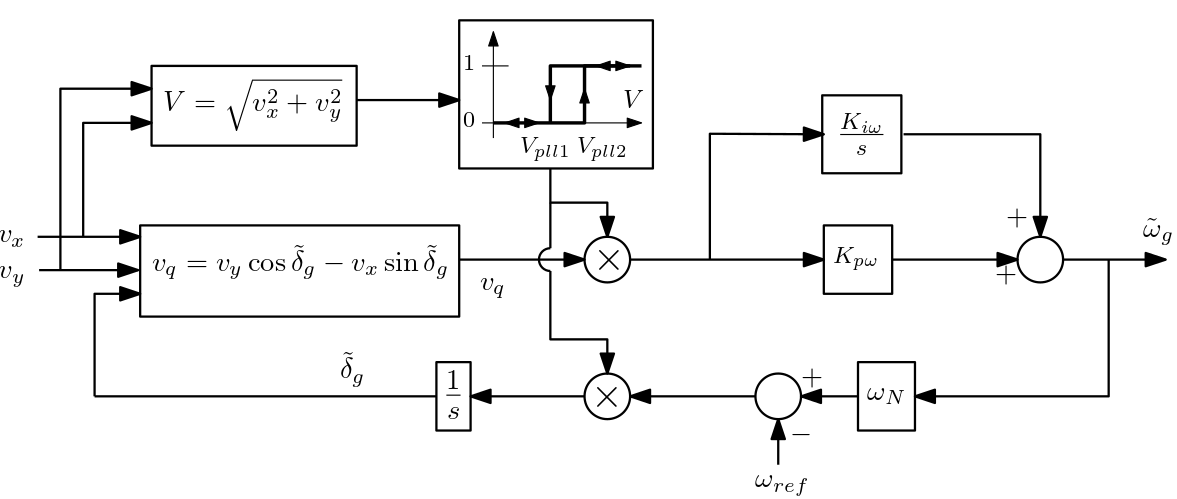
\includegraphics[width=0.8\textwidth]{inj_gfol_pll.png}
\end{center}

{\bf Inner current control.} PI controllers with cross-coupling compensation
give the modulated voltage:
\[
v_{md} = \frac{v_d}{r} - \tilde\omega_g L\, i_q
 + \Big(K_p + \frac{K_i}{s}\Big)\big(i_d^{ref} - i_d\big),
\qquad
v_{mq} = \tilde\omega_g L\, i_d
 + \Big(K_p + \frac{K_i}{s}\Big)\big(i_q^{ref} - i_q\big)
\]
\begin{center}
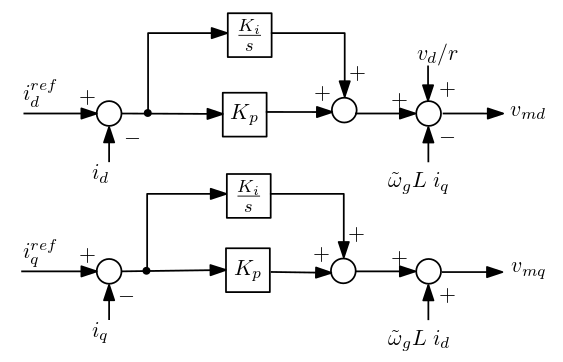
\includegraphics[width=0.55\textwidth]{inj_gfol_currentctl.png}
\end{center}
combined with the transformer relationship
$v_{md} = v_d/r + R\, i_d - \tilde\omega_g L\, i_q$,\ \
$v_{mq} = v_q/r + R\, i_q + \tilde\omega_g L\, i_d$.

\newpage

{\bf Active power control.} The measured power is filtered ($T_{lpf}$) and
compared with the setpoint $P^0$; a PI controller ($K_{pp}$, $K_{ip}$) with
non-windup limits $\pm I_d^{max}$ produces $i_d^{ref}$. Priority is given to
the reactive current:
\[
I_d^{max,stat} = \sqrt{\max\big(I_{max}^2 - i_q^2,\ 0\big)}
\]
and $I_d^{max}$ tracks this value through a first-order lag ($T_{rlim}$,
typically 0.002~s) with rate limits {\tt dPdt\_min}/{\tt dPdt\_max}, limiting
in particular the rate of recovery of the active current after it has been
decreased owing to an increase of $i_q$.
\begin{center}
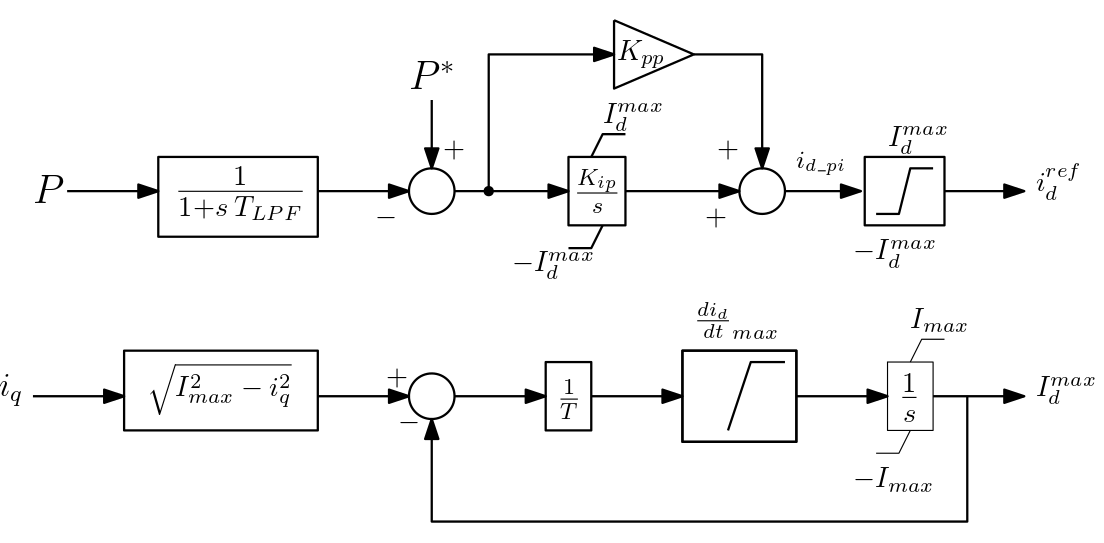
\includegraphics[width=0.8\textwidth]{inj_gfol_pctl.png}
\end{center}

{\bf Voltage / reactive power control.} Depending on {\tt vqswitch}, either
the compensated voltage $V_c = \big|\bar v/r + (R_c + jX_c)\,\bar\imath\,\big|$
({\tt vqswitch}=1) or the reactive power $Q$ ({\tt vqswitch}=0) is controlled.
The controlled quantity is filtered ($T_{lpf}$) and its deviation from
setpoint drives a PI controller ($K_{pv}$, $K_{iv}$) with non-windup limits
$\pm i_{q1}^{max}$, giving $i_{q1}$; the error is zeroed (controller frozen)
while $V < V_{s2}$. Dynamic voltage support adds a component $i_{q2}$,
piecewise linear in $V$: zero above $V_{s1}$, decreasing linearly to
$-I_{max}$ at $V_{s2}$, constant below. The total $i_{q1}+i_{q2}$, limited to
$\pm I_{max}$, is the reference $i_q^{ref}$.
\begin{center}
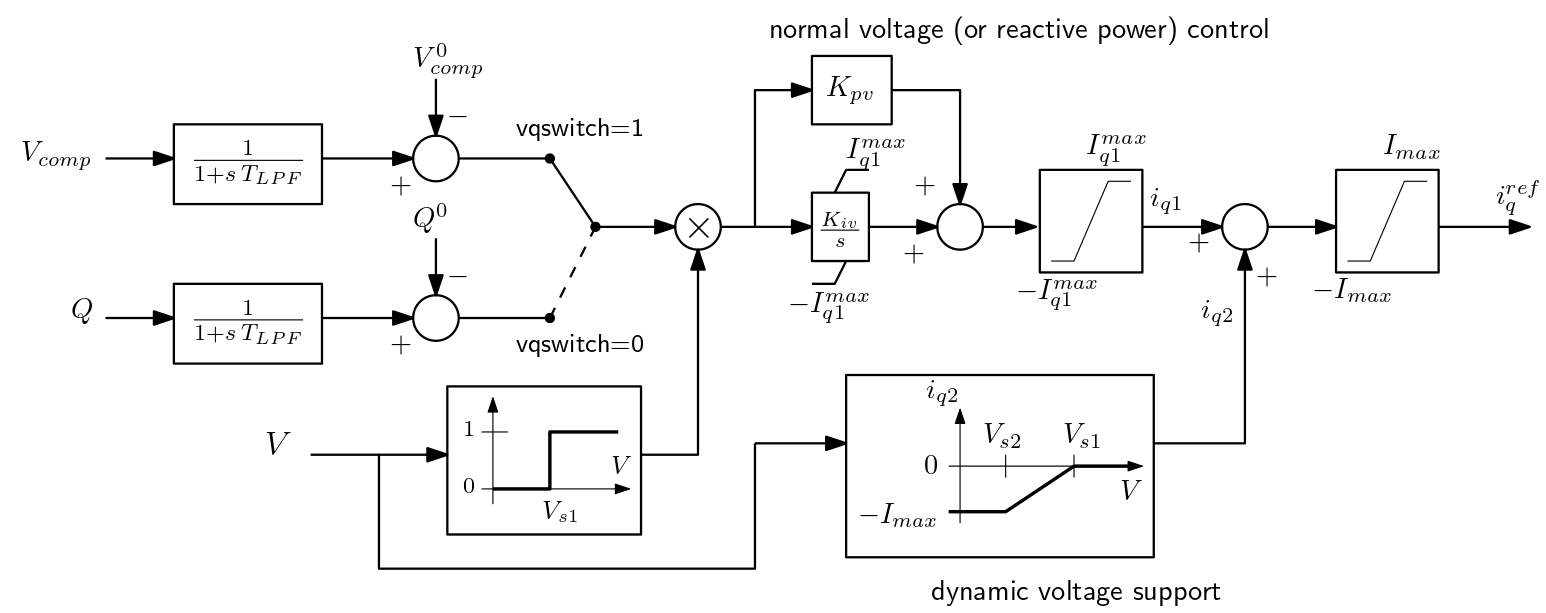
\includegraphics[width=0.9\textwidth]{inj_gfol_qctl.png}
\end{center}
With $R_c = R$, $X_c = \omega L$ and $r=1$, the magnitude of the modulated
voltage is controlled.

\newpage

{\bf Data.} The record has the following structure (defaults from the
{\tt Benchmark\_1\_VSC} test case distributed with RAMSES):

{\tt INJEC GFOL NAME BUS FP FQ P Q\ \ R L r Snom Rc Xc Kp Ki Tlpf Kpp Kip
Trlim dPdt\_min dPdt\_max Kpv Kiv tau Vpllb Vpllu Imax Vs1 Vs2 iqmax
vqswitch ;}

\begin{center}
\begin{tabular}{llll}
\hline
Parameter & Description & Unit & Default \\
\hline
{\tt R}        & phase reactor resistance                        & pu   & 0.005  \\
{\tt L}        & phase reactor inductance                        & pu   & 0.15   \\
{\tt r}        & ratio of ideal transformer                      &      & 1.02   \\
{\tt Snom}     & nominal apparent power                          & MVA  & 1200   \\
{\tt Rc}       & resistance used in compensated voltage          & pu   & 0.005  \\
{\tt Xc}       & reactance used in compensated voltage           & pu   & 0.15   \\
{\tt Kp}       & current control: proportional gain              &      & 0.573  \\
{\tt Ki}       & current control: integral gain                  &      & 6.0    \\
{\tt Tlpf}     & measurement time constant (low-pass filter)     & s    & 0.0033 \\
{\tt Kpp}      & active power control: proportional gain         &      & 0.0333 \\
{\tt Kip}      & active power control: integral gain             &      & 10.0   \\
{\tt Trlim}    & time constant of $I_d^{max}$ rate limiter       & s    & 0.002  \\
{\tt dPdt\_min}& min rate of change of the $d$-current limit     & pu/s & $-999$ \\
{\tt dPdt\_max}& max rate of change of the $d$-current limit     & pu/s & 10.0   \\
{\tt Kpv}      & reactive power control: proportional gain       &      & 0.1667 \\
{\tt Kiv}      & reactive power control: integral gain           &      & 50.0   \\
{\tt tau}      & response time of PLL                            & s    & 0.10   \\
{\tt Vpllb}    & voltage below which the PLL is blocked          & pu   & 0.4    \\
{\tt Vpllu}    & voltage above which the PLL is unblocked        & pu   & 0.5    \\
{\tt Imax}     & maximum current (typically 1--1.2)              & pu   & 1.0    \\
{\tt Vs1}      & voltage below which reactive support starts     & pu   & $-1000$\\
{\tt Vs2}      & voltage of maximum reactive support ($V_{s2}<V_{s1}$) & pu & $-2000$\\
{\tt iqmax}    & limit ($\pm$) on quadrature current $i_{q1}$    & pu   & 1.001  \\
{\tt vqswitch} & 1 = voltage control, 0 = reactive power control &      & 1      \\
\hline
\end{tabular}
\end{center}

Setting {\tt Vs1} and {\tt Vs2} to large negative values (as in the
benchmark) disables the dynamic voltage support. Typical values of
{\tt Kiv} are 50~pu/s for voltage control and 10~pu/s for reactive power
control. The setpoints $P^0$, $Q^0$ and $V_c^0$ are computed at
initialization from the power-flow solution and can be modified during the
simulation with {\tt CHGPRM} disturbances.

Example (from {\tt Benchmark\_1\_VSC}), spanning two lines:

{\tt INJEC GFOL HVDC1 A 1. 1. 0. 0. 0.005 0.15 1.02 1200. 0.005 0.15 0.5730
6. 0.0033 0.0333 10. \\
0.002 -999. 10. 0.1667 50. 0.10 0.4 0.5 1.000 -1000 -2000 1.001 1 ;}

{\bf Observables:} {\tt P\_MW}, {\tt Q\_Mvar}, {\tt Vc}, {\tt Vm},
{\tt vmd}, {\tt vmq}, {\tt I}, {\tt w\_pll}, {\tt theta\_pll\_deg},
{\tt mult\_pll}, {\tt Idmax}, {\tt Md}, {\tt idref}, {\tt id}, {\tt id\_pi},
{\tt iq\_1}, {\tt iq\_2}, {\tt iqref}, {\tt iq}.

\end{document}
